To validate our method we will run the alignment approach of task tree generation against the same case study as Harms et al. did.
The data was collected on an application portal of the university. Figure \ref{fig:screenshotmasterportal} shows a screenshot of the first page of the portal.
After login, users can fill out multiple forms regarding their personal data as well as upload their CVs. The data entered was fully anonymized. 
In this case study 555 user created arround 3635 feasible user sessions. Further details are enlisted in table \ref{tab:casestudy2}.



\begin{table}
	\centering
	 \begin{tabular}{|r|c|}
		   \hline
		      & \textbf{Case Study 2} \\
		      & Application Portal \\
		     \hline
		       Start of Recording & 25 October 2013 \\
		       End of Recordning & 7 March 2014 \\
		       Recorded Users & 555 \\
		       Recorded User Sessions & 4,129 \\
		       Considered User Sessions & 3,635 \\
		       \hline
		         \textbf{Recorded Events} & 350,368 \\
		         Relevant Events & 306,568 \\
		         Double Clicks & 6,437 \\
		         Focus Changes & 89,825 \\
		         \hline
			   \textbf{Considered Events} & 210,306 \\
			   Different Events & 1,897 \\
			   \hline
			    \end{tabular}
			    \caption{Case study overview}
	\label{tab:casestudy2}
\end{table}



Another aspect of our approach we want to examine is the necessity of the calculation of the distance between non-event-tasks. 
The calculations of those distances are very expensive operations so we are interested if this step could be left out and we still find approximatly the same amount of tasks, in the same quality.


\begin{table}
	\begin{tabularx}{\textwidth}{|c|X|c|c|}
	   \hline
		   Parameter & Function & Definition & Used values\\
	     \hline
	       k & The value of the maximum score in the substitution matrix& \ref{def:scorewithmaximalscore}& 6 \\
	       L & Penalty for the score between non-event-tasks & \ref{def:scoreadjusted} & 3\\
	       T & Threshold score for determination of match importance & \ref{def:treshold} &9\\
	       g & Gap penalty for inserting gaps & \ref{def:gappenalty} &3\\
	       f & Number of occurrences a task must at least have in all user sessions to be replaced & \ref{def:minoccurrencecount} &3\\
	       \hline
 \end{tabularx}
 \caption{Table of all parameters of the sequence detection.}
 \label{tab:parameters}
 \end{table}


\begin{itemize}
	
	\item Two case studies: 
		\begin{itemize}
			\item Application portal case study. 
			\item Website of research group
		\end{itemize}
	\item Table of Case studies
	\item Screenshot of Application Master Portal
	\item Screenshot of Website of research group
	\item Show XML recorded traces
	\item When running the full case study alot of perfomance problems came up.
	\item Memory consumption and computation time grew alot due to the nature of the algorithm
	\item Computation moved from a Intel(R) Core(TM) i5-2520M CPU @ 2.50GHz with 8GB Ram to a AMD Opteron(TM) Processor 6276 (64 core) with 250GB Ram.
	\item The java virtual machine was given 64GB
	\item Still computation time extremly large (see performance evaluation)
	
	\item Maybe change stop criterium: 10% of the matches found in the first run
	\item Other solution: Update substution matrix, so non-Event tasks can have a negative score (less likely to find matches then)
\end{itemize} 

\section{Data Preprocessing}
After loading the input data from all XML files the following preprocessing steps have been performed. The information about each command is copied from its man page in AutoQUEST.
\begin{itemize}
	\item condenseHTMLGUIModel: Merges all equal nodes in the GUI-Model.
	\item condenseMouseClicks: Reduces a sequence of mouse button down, mouse button up and mouse click with the same button on the same event target to a single mouse click with that button on that target. The mouse button down and mouse button up events are discarded.
	\item correctKeyInteractionTargets: Iterates the provided sequences and sets the target of all key interaction events to the GUI element having the current keyboard focus. The current keyboard focus is determined either by keyboard focus events or by using the target of the first key interaction in a sequence. Events changing the keyboard focus are discarded herewith.
	\item correctTabKeyNavigationOrder: Iterates the provided sequences and corrects the order of events in case of tab key navigation. This is required, as from time to time the event of pressing the tab key for navigation in formulars comes before the text input event in a text input field out of which the tab key navigates.
\end{itemize}

\section{Evaluation of termination conditions}
\begin{itemize}
	\item Run CTA with full case study
	\item show matches found per iteration and time per iteration

	\begin{table}
		\centering
	\begin{tabular}{|c|r|c|c|}
		  \hline
		  Iteration & Matches & Absolute time& Relative time \\
		  \hline
     		    0  & 1,112,794 & 26.17 & 26.17\\
	            1  & 381,190   & 39.16 & 12.99\\
		    2  & 167,677   & 45.52 & 6.36\\
		    3  & 63,964    & 51.00 & 5.48\\
		    4  & 26,171    & 55.83 & 4.83\\
		    5  & 12,627    & 60.72 & 4.89\\
		    6  & 8,660     & 65.48 & 4.76\\
		    7  & 7,517     & 70.34 & 4.86\\
		    8  & 7,232     & 75.02 & 4.68\\
		    9  & 7,214     & 79.74 & 4.72\\
		    10 & 7,214     & 84.49 & 4.75\\
		  \hline
		   \end{tabular}
		   \caption{Matches found per iteration and the time for each iteration. All times in minutes.}
		   \label{tab:timesandmatchesperiteration}
	\end{table}

	\begin{figure}
		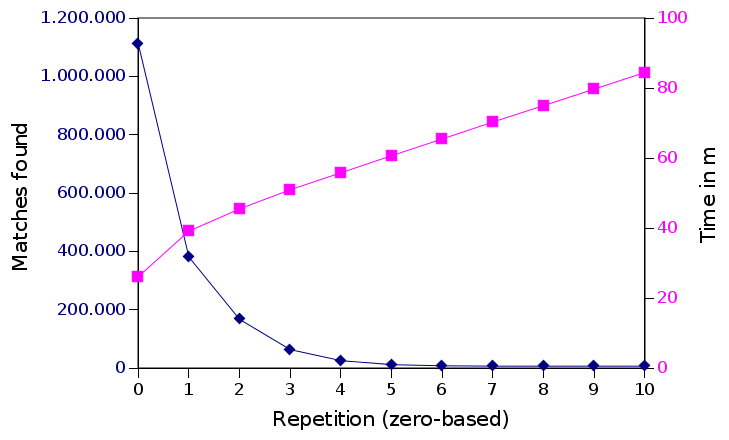
\includegraphics[width=\textwidth]{chapters/casestudy/hasehase.png}
		\caption{}
		\label{fig:hasehase}
	\end{figure}
\end{itemize}

\section{Calculation of distances between non-Event-Tasks}

\section{Performance Evaluation}
\begin{itemize}
	\item Compare Core-TaskTrees(CT) with Core-TaskTrees-Algignment (CTA)
	\begin{itemize}
		\item Run CT with 10, 100, 1000, all user sessions on CS1
		\item Run CTA with 10, 100, 1000, all user sessions on CS1
		\item Show percentage of each step of CTA of all user sessions
		\item Run CT with 10, 100, 1000, all user sessions on CS2
		\item Run CTA with 10, 100, 1000, all user sessions on CS2
		\item Show percentage of each step of CTA of all user sessions
	\end{itemize}
	\item Alot of tables (which step of the algorithm takes how long, for each dataset
\end{itemize}

\section{Generated Task Trees}
\begin{table}
 \begin{tabular}{|r|c|c|}
	   \hline
	      & \textbf{Harms et al.} & \textbf{Alignment approach} \\
	     \hline
	       \textbf{Generated Tasks} & 10,634 & 6,532 \\
	       Sequences & 9,530 & 2,759 \\
	       Iterations & 1,104 & 619 \\
	       Selections & -& 1,156 \\
	       Optionals & -& 101 \\
	       \hline
\end{tabular}
\end{table}


\begin{itemize}
	\item Show some meaningful generated task trees
	\item Show also tasktrees that are not useful
\begin{figure}
	\centering
	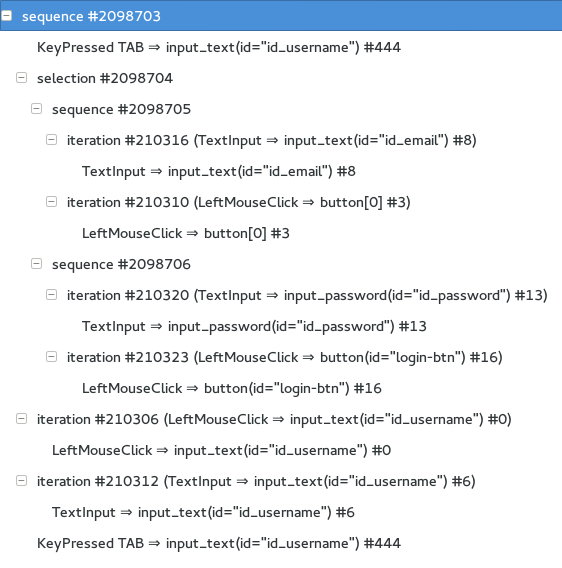
\includegraphics[]{chapters/casestudy/mixedtasktree.png}
	\caption{}
	\label{}
\end{figure}
\begin{figure}
	\centering
	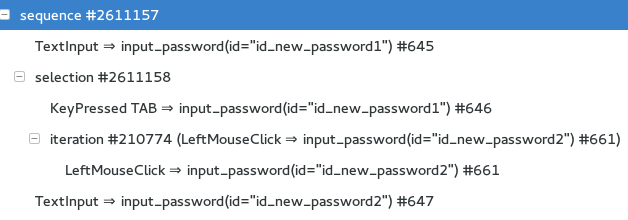
\includegraphics[]{chapters/casestudy/newpassword.png}
	\caption{}
	\label{}
\end{figure}
\begin{figure}
	\centering
	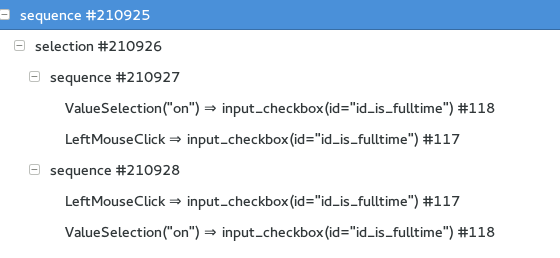
\includegraphics[]{chapters/casestudy/preprocessing_needed.png}
	\caption{}
	\label{}
\end{figure}
\begin{figure}
	\centering
	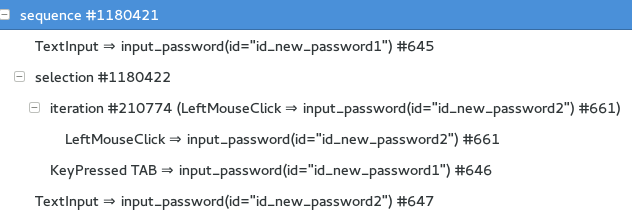
\includegraphics[]{chapters/casestudy/newpassword-1.png}
	\caption{}
	\label{}
\end{figure}
\begin{figure}
	\centering
	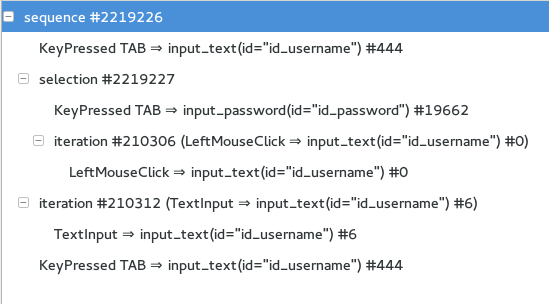
\includegraphics[]{chapters/casestudy/login_process_repeated.png}
	\caption{}
	\label{}
\end{figure}
%\begin{figure}
%	\centering
%	\includegraphics[]{}
%	\caption{}
%	\label{}
%\end{figure}
\end{itemize}


\section{Discussion}
\begin{itemize}
	\item Task Graph
\end{itemize}
